\documentclass[12pt]{article}
\usepackage[utf8]{inputenc}
\usepackage{geometry}
\usepackage{graphicx}
\usepackage{amsmath}
\usepackage{amssymb}
\usepackage{hyperref}
\usepackage{cleveref}
\usepackage[backend=biber, sorting=none, style=ieee]{biblatex}
\addbibresource{main.bib}

\geometry{a4paper, margin=1in}

\title{A Cloud-Based Solution for Efficiently Processing and Storing Highway Camera Logs}
\author{Casper Kristiansson \and Nicole Wijkman}
\date{\today}

\begin{document}

\maketitle

\section{Context}\label{context}
As every day passes the effectiveness and usage of data continue to grow rapidly, especially in areas of our daily life. One such domain is traffic management solutions where the efficient use of technology can improve the experience for millions of people. The United States of America has an active proposal called 511 Travel Information Telephone Services \cite{dotFHWATravel} that provides traffic information to its citizens. This has enabled approximately 90\% of the states to offer web applications for real-time highway camera viewing \cite{fl511FL511}.

PKTraffic LLC. \cite{pktrafficPKTraffic} is a company that uses these cameras to capture and collect traffic data more specifically incident data. Their system is developed to efficiently and accurately collect vast amounts of data using a low-cost solution, enabling it to broaden its impact and provide a sought-after service for multiple entities.

The issue with highway cameras is that a large majority of them receive issues like 404 not found, 503 service unavailable, and a lot of other errors. Because the company collects footage from around 2,000-2,500 cameras the logs generated from all of them are quite large. In their current situation, PKTraffic doesn't have any good system in place for storing the logs in a manner so that they can easily be accessed, managed, and visualized.

\section{Solution}
The company PKTraffic currently is using a hybrid tech solution using both cloud products from Amazon AWS  \cite{CloudSer68:online} and a local server. Because of this the data collection and management will be developed using AWS services like DynamoDB \cite{FastNoSQ49:online}, kinesis streams \cite{Processa96:online}, and Lambda \cite{Serverle45:online}.

\subsection{Data Collection}
The data collection part of the program as mentioned from the context (section  \ref{context}) comes from traffic highway cameras. While the actual recording of the cameras generates a lot of logs like bytes from each request, camera information, etc. we are mostly interested in the HTTP requests made. The Goal with logging is to keep track of whether the application has successfully been capturing footage and whenever it has not been able to do it.

This means that before the application starts capturing footage we want to capture the current time and send a put log event. We then wait until the camera recording has stopped and log the reason for stopping whenever it is an expected or unexpected error.

\subsection{Data Management}
The data management part of the program is the actual part that manages the incoming data from the data collection. It mainly consists of two parts; a Kinesis data stream to collect and batch the data together and a Lambda script to process the data.

\subsubsection{Amazon Kinesis Data Streams}
The setup for a kinesis stream was extremely easy which consisted of simply creating the stream with few configurations like setting the data retention period to 24 hours and enabling on-demand mode. After completing this we can then in the python script simply use boto3 \cite{Boto312825:online} client to put an event to the kinesis stream.

\subsubsection{Amazon Lambda Functions}
After events have been written to the kinesis data stream we need some way to analyze and manage the data. Using AWS lambda we can easily specify a trigger for the kinesis data stream like the batch size (amounts of events) or batch window. Using these settings we can easily group the logged data and perform the required analytics of the data. In our case, we want to perform two specific actions. The first one is to store the logged event in dynamoDB and the second is to update the latest status of the camera. Both of these actions are easy insertions into two different tables. This structure is also future-proof to help with any future analytics that might want to be performed on the logged data.

\subsubsection{Amazon DynamoDB and MySQL}
The storing of the data consists of two different database types. The first one is a NoSQL database using dynamoDB and a relational database using MySQL. The NoSQL database is used to keep track of all logged events while the NoSQL database will manage the latest status of each camera.

The reason for dividing the databases is due to performing the query to get the latest status of all of the cameras would be extremely slow and costly due to the structure of the tables.

The dynamoDB table consists of three different columns; cameraId (PK), timestamp (SK), and a status code. The status code is a simple integer that maps back to a dict which contains the specific error code. The reason for mapping the status code instead of saving the entire error in the database has to do with lowering the cost. By using this structure each item comes down to 33.7 bytes which means that storing a total of ~267,000 logs results in a table size of 8 MB. Using this type of PK and SK system enables fast queries to extract logs for a given camera in a specific date range.

Lastly, the MySQL database will consist of one entry for each camera. The table will save the same information as the dynamoDB items which are the camera, last updated, and status. Using a second table for the status means that we can easily query the entire table to get the status of all cameras.

\subsection{Data Visualization}
The data valuation part of the program consists of a lambda endpoint for querying the data and a React.js \cite{React40:online} application for visualization. The objective of this project was to create two dashboards: one showing the current status of all cameras on a map, and another for simulcasting a specific camera's uptime over a certain time span. However, due to time constraints, only the dashboard for visualizing a specific camera was completed.

\subsubsection{Backend - AWS Lambda}
The AWS lambda was created using Python and deployed using Serverless \cite{Serverle24:online}. The Python scripts execute two queries: the first extracts all logs within a specified date range, while the second retrieves the earliest event that predates that range. The script then has a bit of logic for grouping the data before it is returned to the frontend.

\subsubsection{Frontend - React.js}
The frontend part of the project was developed on an existing project. This means that by simply creating a new page we accept two different inputs which are a specific camera ID and a date. We then can simply generate horizontal timelines displaying either green when a camera was recording or red whenever the camera was not recording.

\begin{figure}[!h]
    \centering
    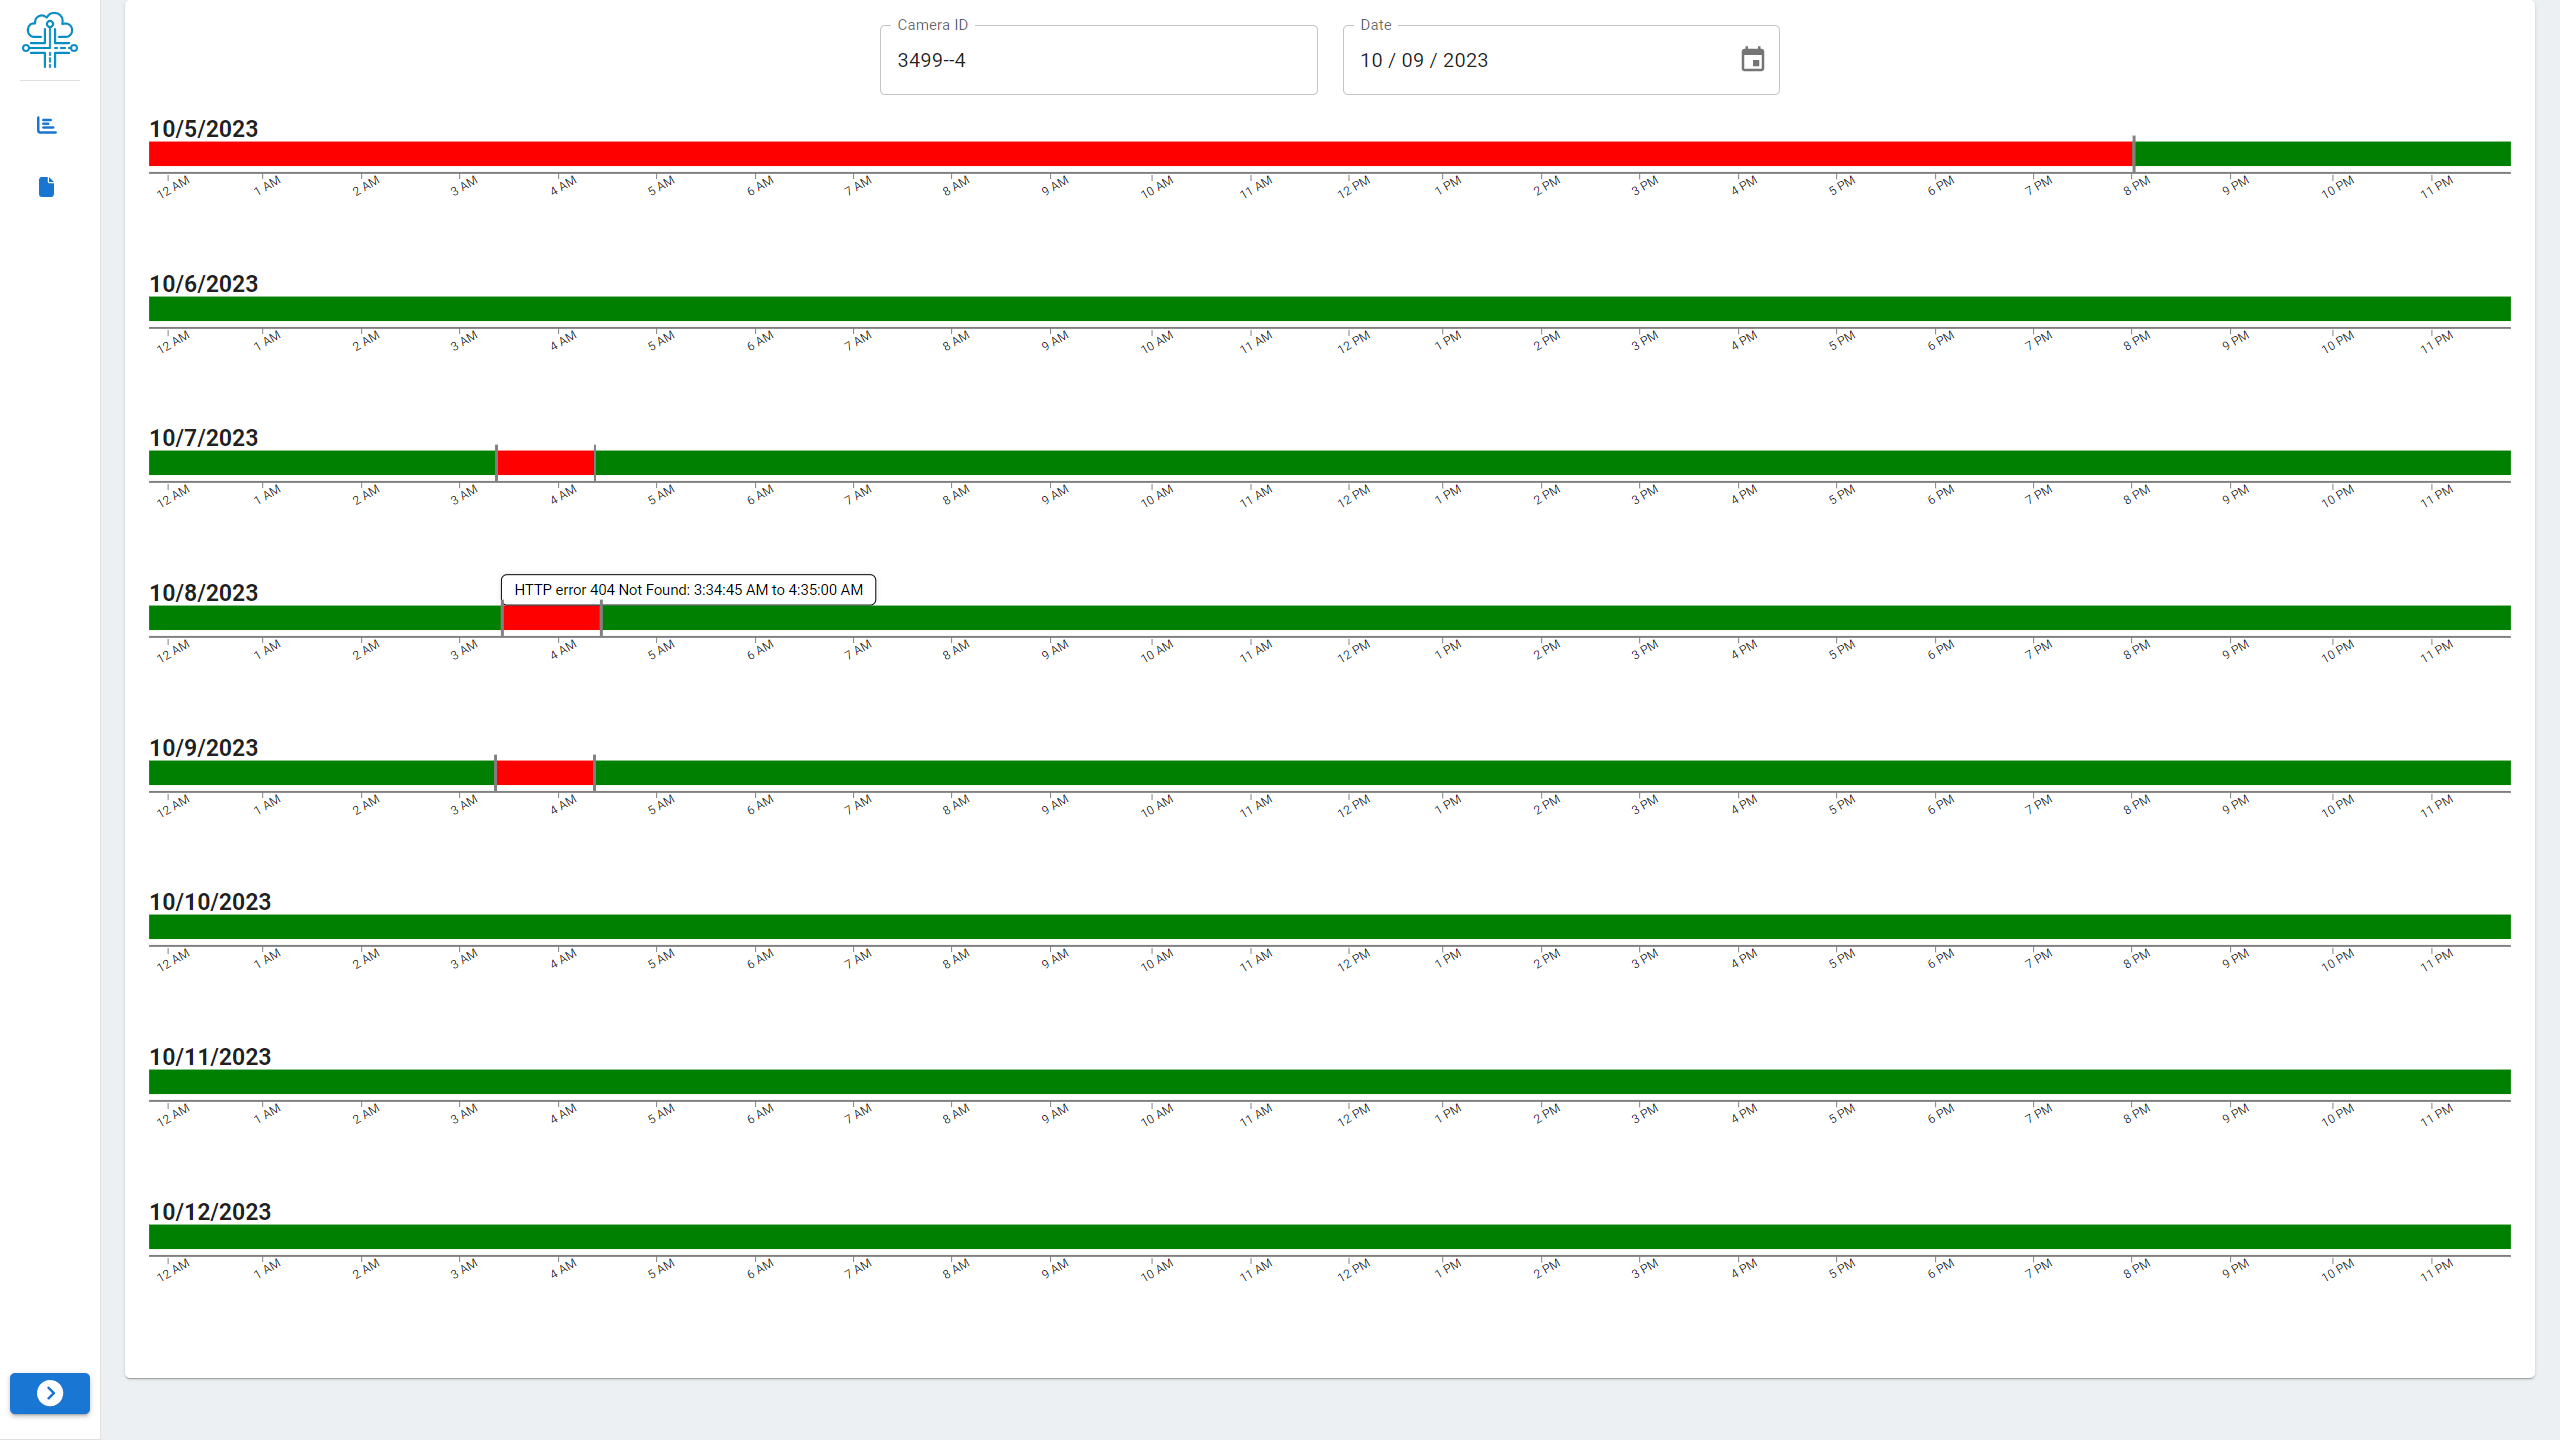
\includegraphics[width=1\linewidth]{dashboard.jpg}
    \caption{The dashboard displaying a camera uptime}
    \label{fig:enter-label}
\end{figure}

\section{Result}
The entire workflow from logging a specific event to visualizing it was successful. Using this kind of structure enables an efficient way to manage events that will be able to manage the required workflows of 50,000 - 100,000 highway cameras. The solution was built using AWS products that are still able to operate at a really low cost.

The Notebook.pdf contains the code and a more detailed description of everything that has been done in this project. While as discussed due to time constraints the dashboard for visualizing a map of the latest status of all cameras wasn't completed the dashboard for viewing a specific camera was. The backend structure for the map visualization is completed and therefore can easily be implemented in the future.

\printbibliography

\end{document}
